\documentclass[spec, och, labwork]{shiza}
% параметр - тип обучения - одно из значений:
%    spec     - специальность
%    bachelor - бакалавриат (по умолчанию)
%    master   - магистратура
% параметр - форма обучения - одно из значений:
%    och   - очное (по умолчанию)
%    zaoch - заочное
% параметр - тип работы - одно из значений:
%    referat    - реферат
%    coursework - курсовая работа (по умолчанию)
%    diploma    - дипломная работа
%    pract      - отчет по практике
% параметр - включение шрифта
%    times    - включение шрифта Times New Roman (если установлен)
%               по умолчанию выключен
\usepackage{subfigure}
\usepackage{tikz,pgfplots}
\pgfplotsset{compat=1.5}
\usepackage{float}

%\usepackage{titlesec}
\setcounter{secnumdepth}{4}
%\titleformat{\paragraph}
%{\normalfont\normalsize}{\theparagraph}{1em}{}
%\titlespacing*{\paragraph}
%{35.5pt}{3.25ex plus 1ex minus .2ex}{1.5ex plus .2ex}

\titleformat{\paragraph}[block]
{\hspace{1.25cm}\normalfont}
{\theparagraph}{1ex}{}
\titlespacing{\paragraph}
{0cm}{2ex plus 1ex minus .2ex}{.4ex plus.2ex}

% --------------------------------------------------------------------------%


\usepackage[T2A]{fontenc}
\usepackage[utf8]{inputenc}
\usepackage{graphicx}
\graphicspath{ {./images/} }
\usepackage{tempora}

\usepackage[sort,compress]{cite}
\usepackage{amsmath}
\usepackage{amssymb}
\usepackage{amsthm}
\usepackage{fancyvrb}
\usepackage{listings}
\usepackage{listingsutf8}
\usepackage{longtable}
\usepackage{array}
\usepackage[english,russian]{babel}

% \usepackage[colorlinks=true]{hyperref}
\usepackage{url}

\usepackage{underscore}
\usepackage{setspace}
\usepackage{indentfirst} 
\usepackage{mathtools}
\usepackage{amsfonts}
\usepackage{enumitem}
\usepackage{tikz}
\usepackage{minted}
\usepackage{pdfpages}
\newcommand{\eqdef}{\stackrel {\rm def}{=}}
\newcommand{\specialcell}[2][c]{%
\begin{tabular}[#1]{@{}c@{}}#2\end{tabular}}

\renewcommand\theFancyVerbLine{\small\arabic{FancyVerbLine}}

\newtheorem{lem}{Лемма}

\begin{document}

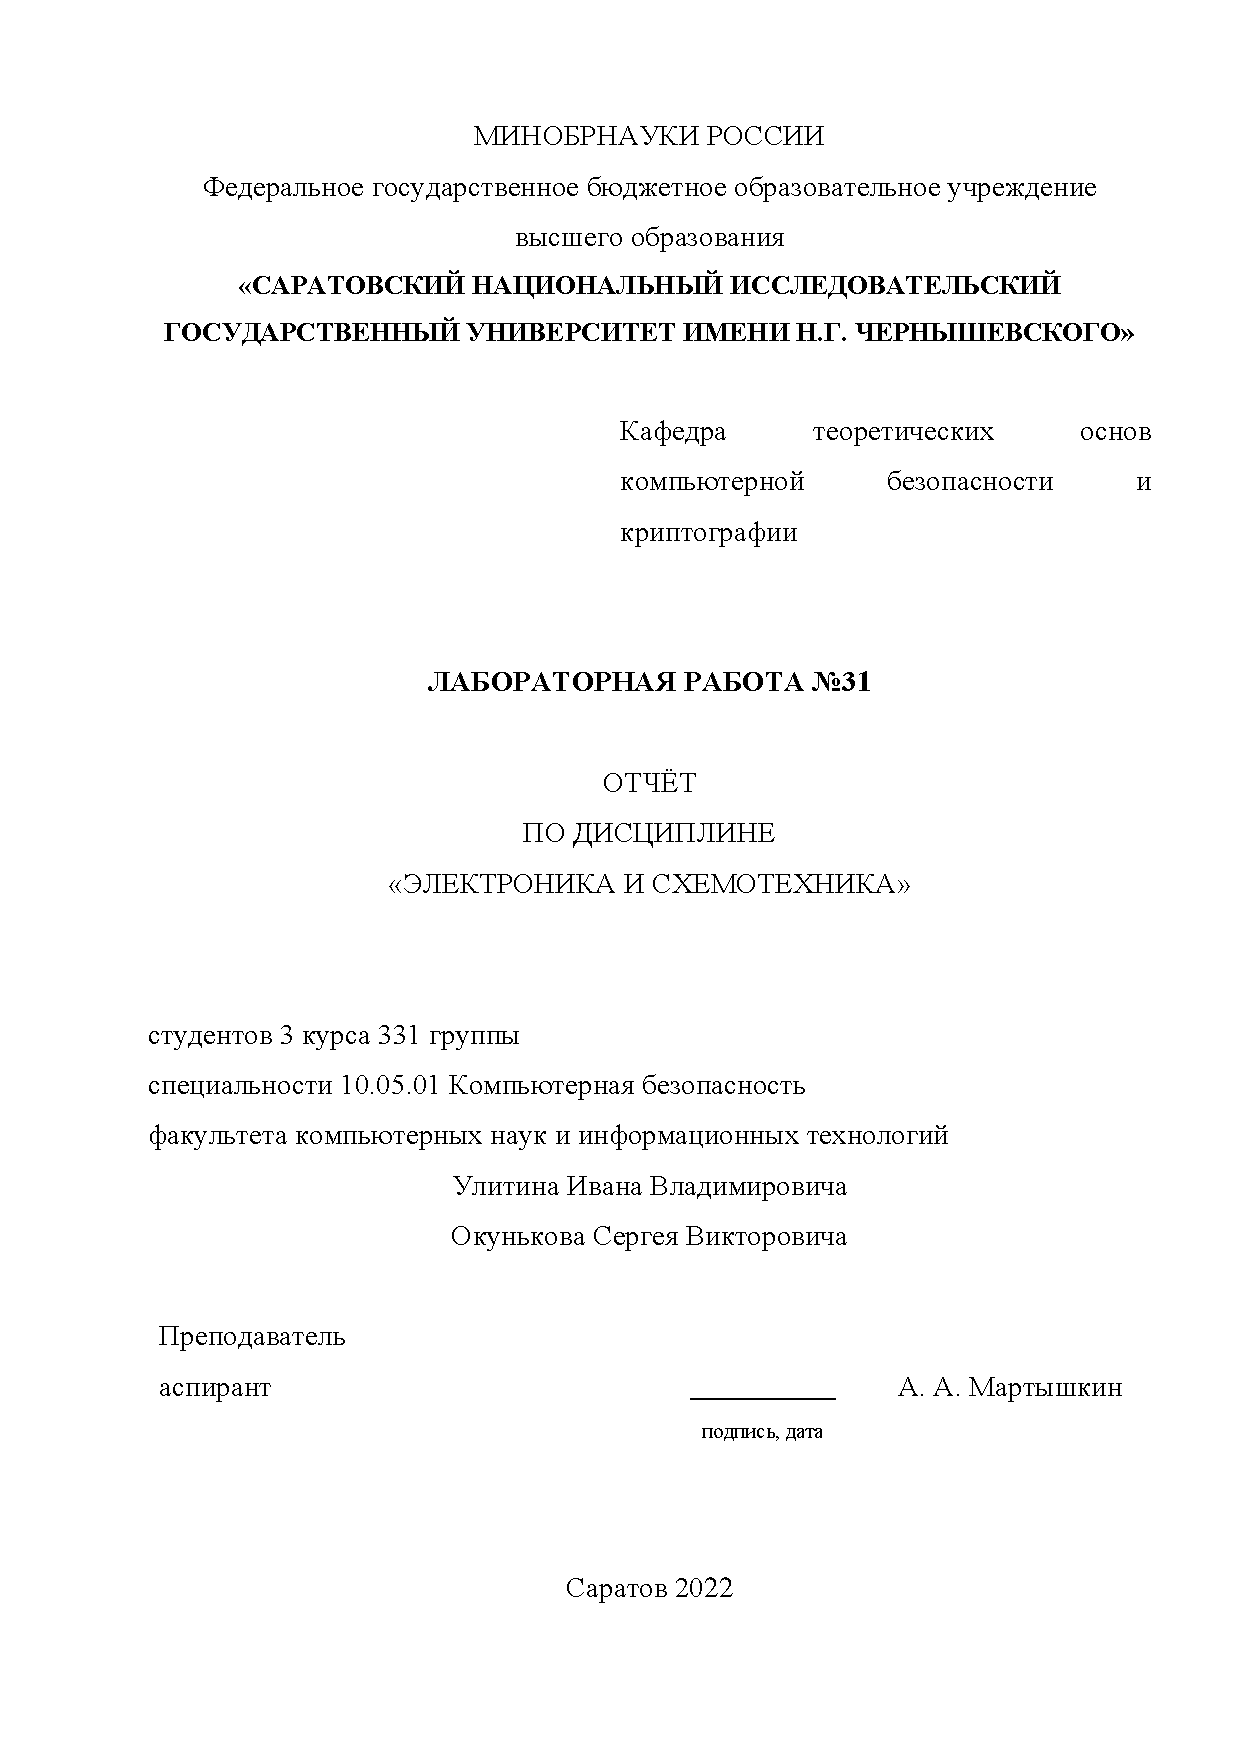
\includepdf{tit31.pdf}

%-------------------------------------------------------------------------------

\textbf{Цель работы:} Ознакомление с основными характеристиками и испытание интегрального цифрового компаратора.

\textbf{Задание 1:}\\
Реализуем схему цифрового компаратора:

\begin{figure}[H]
    \centering
    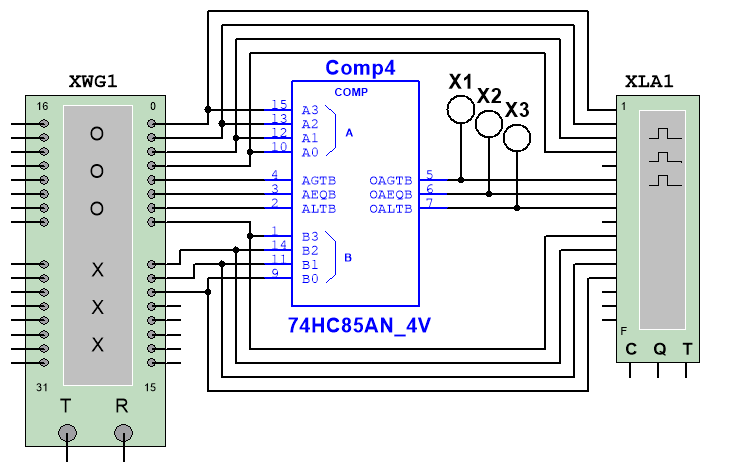
\includegraphics[width=0.8\textwidth]{pic3/1.png}
    \caption{Цифровой компаратор}
\end{figure}

\textbf{Задание 2}\\

По результатам моделирования получим следующую диаграмму входных и выходных сигналов:

\begin{figure}[H]
    \centering
    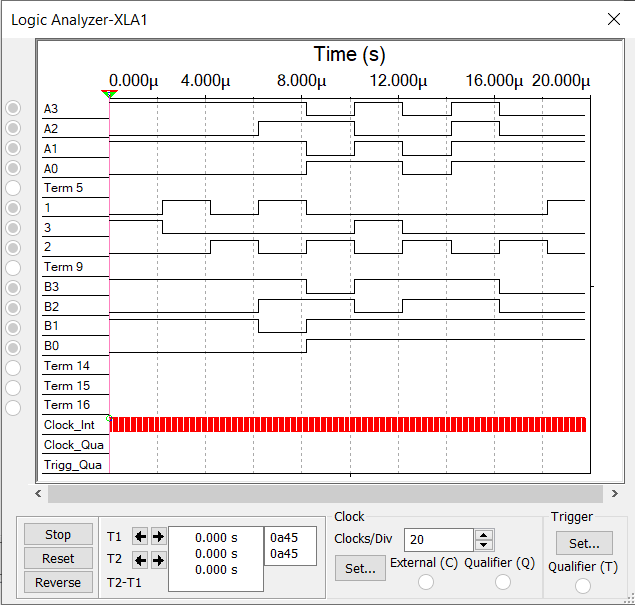
\includegraphics[width=0.8\textwidth]{pic3/2.png}
    \caption{Изображение логического анализатора}
\end{figure}

\begin{figure}[H]
    \centering
    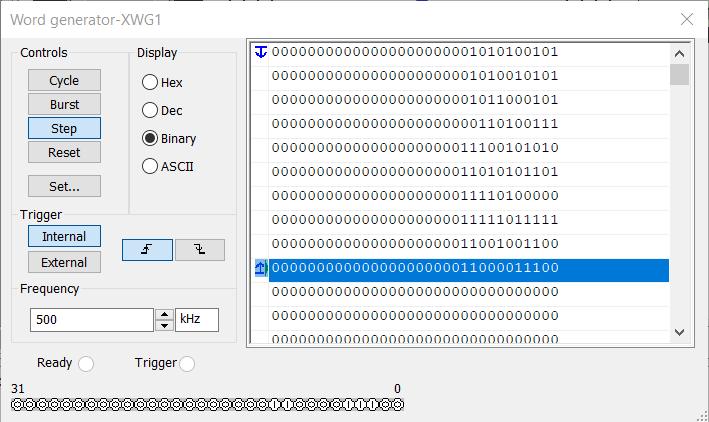
\includegraphics[width=0.8\textwidth]{pic3/3.png}
    \caption{Изображение окна генератора слов XWG1}
\end{figure}

\textbf{Вывод: } ознакомились с основными характеристиками и испытали интегральный цифровой компаратор.

\textbf{Тестовые задания:}\\

\textbf{Задание 1}\\
    Укажите:
    
    \begin{enumerate}
        \item[a)] можно ли установить факт равенства двухразрядных бинарных чисел $A$ и $B$ с помощью приведенного
        устройства сравнения;

        \item[б)] какой \textbf{уровень} сигнала установится на его выходе при равенстве чисел $A$ и $B$ (рис. ниже);

    \end{enumerate}
    
    \begin{figure}[H]
        \centering
        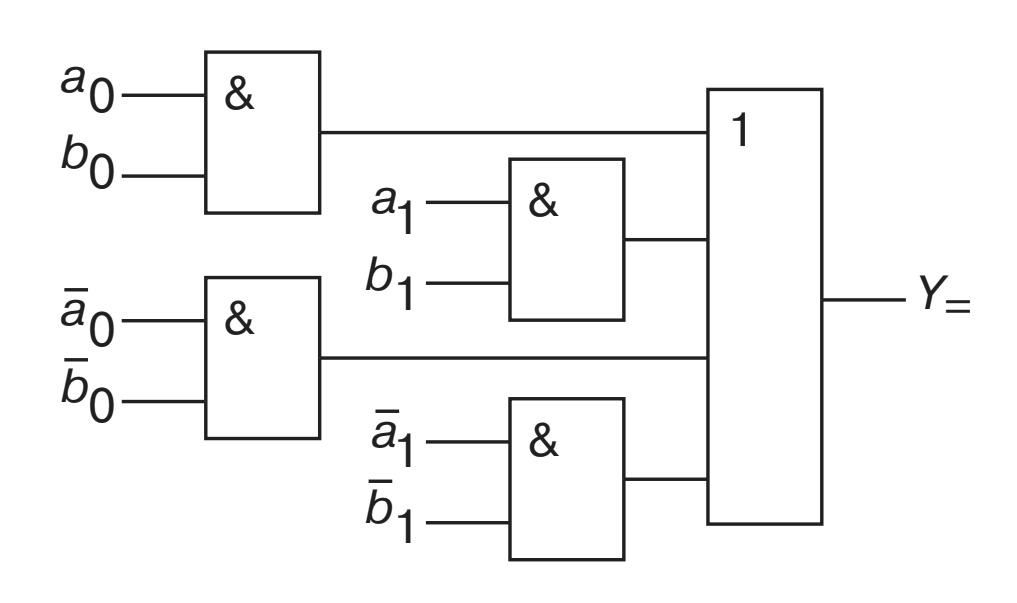
\includegraphics[width=0.5\textwidth]{pic3/test1.png}
        \caption{}
    \end{figure}

    Ответы:
    \begin{enumerate}
        \item[а)] да;
        \item[б)] 1;
    \end{enumerate}

\textbf{Задание 2}\\
    Укажите, какую \textbf{функцию} выполняет цифровой компаратор:
    
    Ответ: сравнение двух бинарных чисел $A$ и $B$ одинаковой разрядностью с целью определения равенства $A = B$ или
    неравенства $A < B$ и $A > B$.

\textbf{Задание 3}\\
    Укажите \textbf{логическую функцию}, выражающую равенство $i$-х разрядов двоичных чисел:

    Ответ: $y = a_i b_i + \overline{a_i b_i}$.
    
\textbf{Задание 4}\\
     Укажите, к какому \textbf{типу} цифровых устройств относят компараторы: 

     Ответ: к комбинационным.

\textbf{Задание 5}\\
    Укажите \textbf{число активных} логических сигналов, формирующихся на выходе компаратора при сравнении многоразрядных двоичных чисел:

    Ответ: 1.
    
\textbf{Задание 6}\\
    Укажите, чем определяется \textbf{число входов} цифрового компаратора:

    Ответ: число входов определяется разрядностью сравниваемых бинарных чисел.
    
\textbf{Задание 7}\\
    Укажите, можно ли построить устройство сравнения требуемой разрядности, используя цифровые компараторы с
    ограниченной разрядностью (например, четырехразрядные):

    Ответ: да.

\end{document}